\section{Development approach}
\begin{figure}
\begin{center}
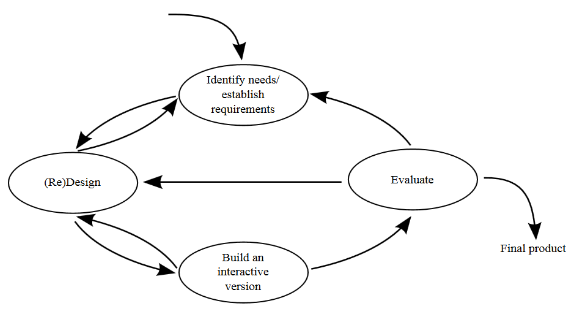
\includegraphics[scale=0.4]{process.png}
\end{center}
\caption{Rogers development process}
\end{figure}
The system was developed using an user centered iterative approach inspired by the development model of Rogers \cite{interaction}, see figure 5,1. This approach puts weight on prototyping and interactions with the client to both identify needs and evaluate prototypes. Thus 3 meetings with a representatives from OM was conducted during the two development iterations.
\section{Overall architecture}
In order to develop a system that fulfils both the functional and nonfunctional requirements, it was decided to develop a web-application in form of a website. Making the system a work as a website will make it highly portable as most client systems have browsers. The system thus becomes a distributed system with a very thin client. The thin client distributed pattern has low complexity as only the presentation layer needs to be distributed, while processing and data is centralized at the server. This ensures data consistency, and allows for a simple and efficient solution. The deployment diagram in figure 5,2 shows the different components of the system and how they are connected. The diagram is split in three parts by the dashed borders. 
Part 1 includes the gathering, formatting and storing of primary building and consumption data to a central database. Meters in OM’s buildings measure the consumption of heat, water and electricity. These informations are depending on the building’s setup, sent through a number of intermediary steps before they reach OM’s current energy management system EnergyKey. Since EnergyKey does not provide any API to access the stored data, the only option was to set it up to export data to an FTP-server. This FTP server is located on an Amazon ec2 instance along with other of BEOVulf’s components. Once EnergyKey uploads data to the FTP-server it will be formatted as csv files.A Java program will start parsing each csv file as soon as it is uploaded and store the data to a central PostgreSQL\footnote{http://www.postgresql.org/} database. More details on this whole process can be found in section \emph{Integration with Energy Key} and \emph{The central database}. Once a batch of new data has been stored in the database the Java program will launch Part 2 of the system.
\begin{figure}
\begin{center}
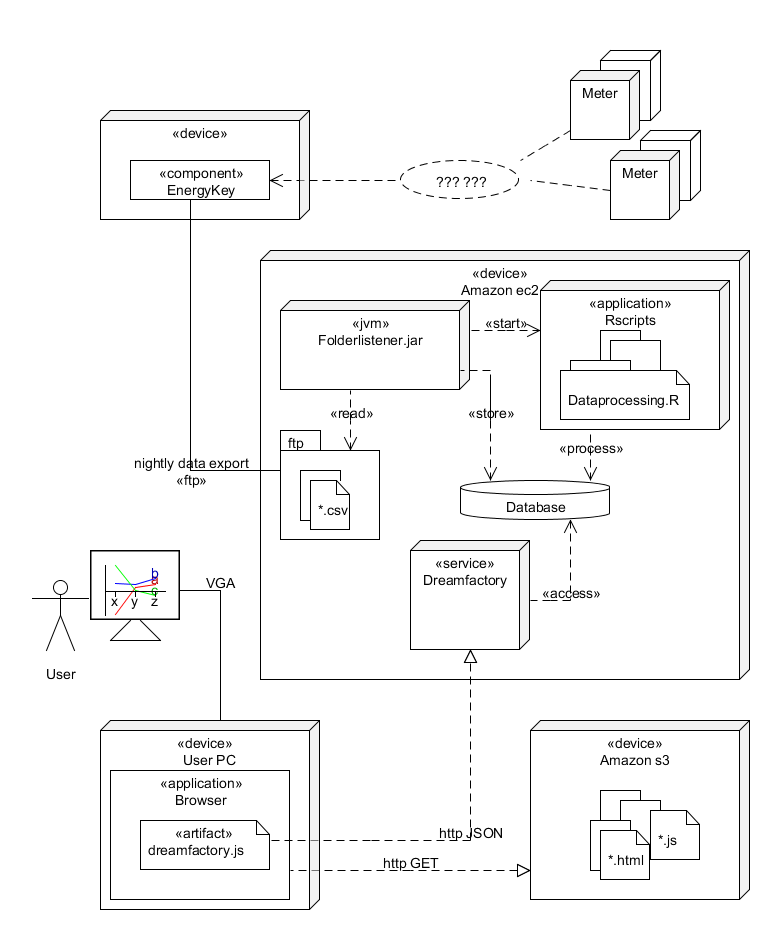
\includegraphics[scale=0.27]{DeploymentDiagramv3.png}
\end{center}
\caption{System deployment diagram}
\end{figure}

Part 2 consists of a number of R\footnote{http://www.r-project.org/} scripts, which will read the raw meter data from the database and perform a number of operations to convert the data into the kind of information that can fulfill the requirements. This includes extracting various features from the consumption, calculating consumption profiles, detecting faults and leakages, comparing buildings and more. Section \emph{Processing Data} describes the details of this process. The results are stored back to the database, where they can be accessed by Part 3 of the system.

Part 3 is the website that users will see, which is hosted in an Amazon s3 bucket\footnote{http://aws.amazon.com/s3/}. The website is powered purely by html and javascript and might be considered static\footnote{http://en.wikipedia.org/wiki/Static\_web\_page}. In order to connect the website with the central database, Dreamfactory has been used. It is a framework for automatically creating a RESTful web service which allows front-end applications to easily connect to the backend. Dreamfactory\footnote{https://www.dreamfactory.com/} exposes the database via a REST API, which uses JSON to transfer data to and from the database. The communication with the database is further simplified by making the website use the Javascript client library provided by Dreamfactory. The design and implementation of the website will be discussed in sections \emph{Design of the Website} and \emph{Implementation of the website}.
\section{Integration with Energy Key}
The integration with Energy Key was done in four main steps. First, a number of exports from Energy Key were made to gather data about buildings their attributes and the which meters are installed in them. Then in step two a year worth of measurements from the meters were exported. In step three the data was cleaned to sort out inconsistencies. And finally in step four a continues flow of data from Energy Key to BEOVulf was set up.
\section*{Step 1 exporting buildings and meters}
The following reports were exported from Energy Key and used to map buildings and meters:
\begin{itemize}
\item Meter list\footnote{Translated from: Målerliste}  (Energy Key $\rightarrow$ Konfiguration $\rightarrow$ Målere $\rightarrow$ Generer rapport)
\item Measurement Reading Report\footnote{Translated from: Aflæsnings Rapport} (Energy Key $\rightarrow$ Aflæsninger $\rightarrow$ Visning $\rightarrow$ Generer rapport)
\end{itemize}
From these reports it was possible to generate a list of all buildings along with a number of attributes such as id, address, name, type (ex. ‘\emph{cultural institution}’) and subtype (ex. ‘\emph{library}’). For each building it was possible to attribute a number of meters which measured either water, electricity or heat. For each meter it was possible to get a installation number, meter number and whatever it was a socalled \emph{billing meter} or \emph{distribution meter}. This attribute is important, because the readings from a \emph{distribution meter} can not be classified as part of the consumption.
\section*{Step 2 - Exporting a year of measurements}
The initial export of measurement data was limited to go one year back, as the data quality declined rapidly when going further back. The exported data was in csv files, one for each meter. The files were thoroughly analysed to determine the structure of the data. Then a Java program was created which could read through the files and insert the measurements in the central database, following the structure described in section \emph{The central database}. The parser made sure that data was consistent, it translated between different units, and if some data did not fit in the program stopped with a warning. The error was examined manually and it was decided what to do with it. Then the parser was changed, the database wiped, and a re-run initiated. This last step was repeated until the parser successfully parsed all 3003 csv files with more than 5.5 million measurements. 
\section*{Step 3 - Detecting errors and cleaning data}
When exporting building data from Energy Key there were unfortunately many buildings with missing attributes, which could not be automatically gathered from anywhere since automated access to the BBR registry is prohibited\footnote{http://bbr.dk/fatibbr}.  Buildings where no type and subtype existed were removed along with all meters belonging to them, while other missing attributes were tolerated. The final amount of buildings in the database was 405. Meters which did not have both installation and meter number were removed, along with meters that had no reported data in the whole exported period. The cleaning reduced the number of meters 33\% from 4293 to 2840 meters. Figure 5.3 shows a table of the final amount of meters stored in the central database:
\begin{figure}
\begin{center}
\begin{tabular}{| l | c | c | r |}
\hline 
  - & Heat & Water & Electricity \\ \hline 
  Total meters & 1282 & 849 & 709 \\ \hline 
  Billing meters in \% & 45\% & 67\% & 97\% \\ \hline
\end{tabular}
\end{center}
\caption{Meters and distribution of type}
\end{figure}

Upon further analysis it was detected that the non automatic meters often had large numbers of overlapping or missing intervals. They were not removed as use cases for them might be found, but data from the non automatic meters was simply too unreliable to be used for advanced calculations and analysis of the building consumption. Therefore a view was created in the database which could filter out non automatic meters, by looking at whatever they have hourly readings or not.
\section*{Step 4 - Continuous meter data collection}
After a year's worth of measurements was initially loaded into the database, a daily export job was created in Energy Key. This export job would automatically export csv files containing the daily measurements to BEOVulf’s FTP-server located on the Amazon ec2 instance. The Java program used to parse the initial batch of measurement data was extended to be able to listen for changes in the folder used by the FTP-server. Once a csv file is fully uploaded to the folder, the java program parses it, puts the measurements contained in it in the database and then archives the csv file. Thus observations from buildings’ meters would come into the database on a daily basis.
\section{The central database}
This section will describe the design of the central database in two parts. The first part is concerned with how the raw data coming from Energy Key is stored, and the second part is about the processed data.
\section*{Raw data}
Figure 5,4 shows an UML diagram of the part of the database, where raw consumption and building data is stored. The main criteria for this design was to be able to store all the data retrieved from Energy Key efficiently without losing any information. The database structure was modeled in a way which is generic enough to capture all kinds of observations without needing a table for each observation. This ensures that whatever data comes from Energy Key could be stored, and the design greatly reduces the number of tables needed. It makes sure that the database complies with the first three normal forms of databases, and the structure makes it possible to treat all measurements the same way when processing data.
\begin{figure}
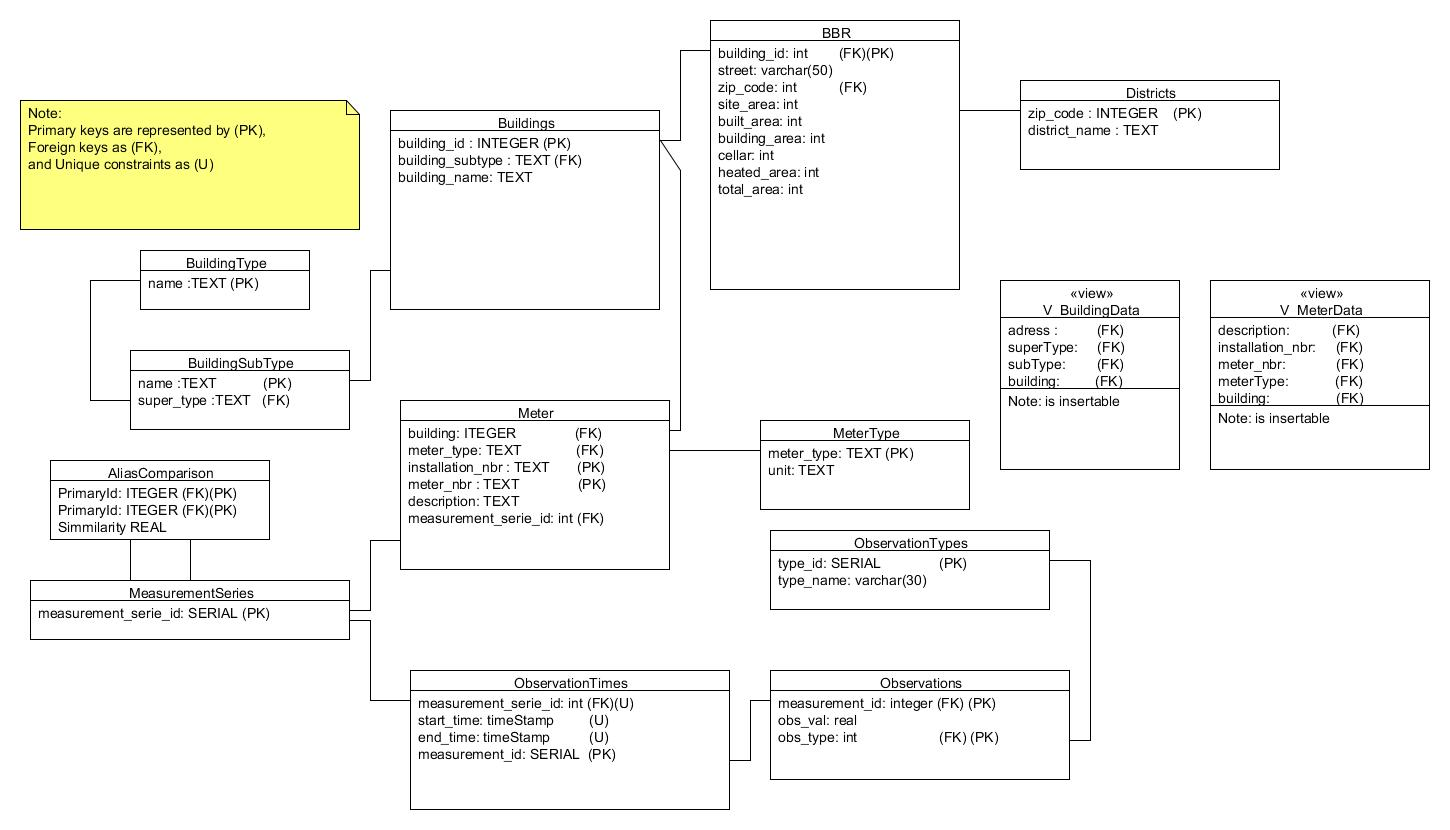
\includegraphics[scale=0.28]{Buildingsdbnew.jpg}
\caption{Database diagram}
\end{figure}
\section*{Buildings and BBR data}
The database contains a table called buildings. Each building has a building\_id, type and subtype which is taken directly from Energy Key. The BBR-table represents the BBR-data collected for each building. This data contains variables like address, building area, site area, cellar size etc. 
\section*{Meters and time series}
When analysing the data, it was found that some buildings had the same physical meter appearing under two or more different installation- and meter numbers, and causing duplicated measurements. The solution was to introduce the \emph{MeasurementSeries} table which represents data from one real physical meter and then map multiple meters from the Meter table to the same measurement serie if they in fact measure the same consumption. Additionally the \emph{AliasComparison} table was created which through a number of triggers and procedures can calculate the similarity between time series of different meters. This enables the database to identify identical meters and dynamically remap meters and series eliminating duplicate time series on a building.
\section*{Observations}
The table Observations, contains all the measured values from all meters. Each record in Observations points to a record in \emph{ObservationType} indicating its type, and to a record in \emph{ObservationTimes} indicating the timeslot in which the consumption was measured. It is possible for many observations thus to point to the same time slot. For example the following observation types can be recorded for a certain time slot when data from a heat meter arrives: in- and outgoing temperature, energy, flow and more.
\section*{Processed data}
Figure 5.5 is a diagram showing the part of the database which stores data that is the result of analyzing and processing the original raw data. The main goal of this design was to make the data as quick to access as possible in the way that it was going to be queried. As an example, all time series data in these tables are stored as arrays with no indication of time nor date, besides a single date in the settings table indicating the start time for all time series. This is because arrays are the most compact representation most compact representation of time series data when transferred in the JSON format used by the website. To further optimize data transfer speeds, all numbers are rounded to a single decimal only.
All tables and views which names are denoted with \emph{W\_*} are used by the website to retrieve information. The \emph{W\_Setings} table, holds configurable settings for both the website and other parts of the system.
\begin{figure}
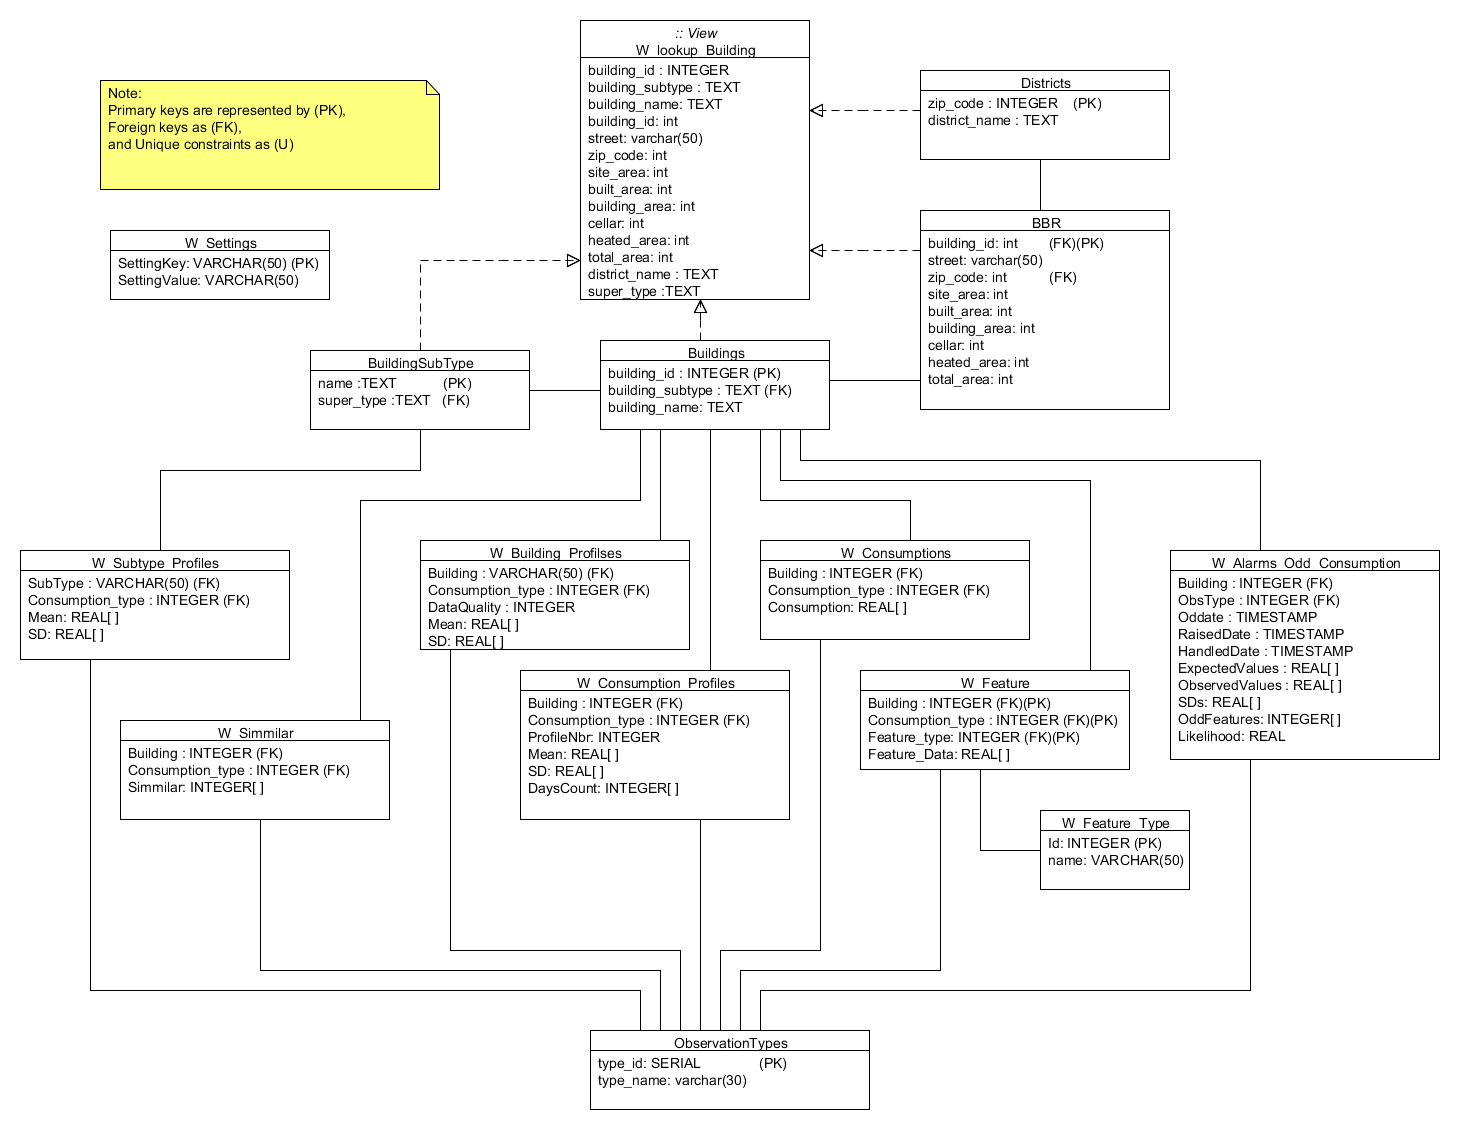
\includegraphics[scale=0.26]{WebSitesidedb.png}
\caption{Database diagram, -Website}
\end{figure}
\section{Processing data}
Processing and analyzing the raw meter data is done by a number of R scripts. The raw consumption data will be loaded from the database into an R session which will do various statistical calculations in order to get useful information from the raw meter data. The R session is launched once a day after new data has arrived, and runs until it has finished processing it. However, some operations are only performed on a weekly basis. The system is designed such that it remains usable while this batch job is running.

The Appendix 07 -Loading data descripes how data is loaded into R and the initial data manipulation.

\section*{Extracting features}
Once the raw consumption is loaded as vectors, the system will convert them to a matrices with 24 columns, one for each hour of the day beginning with 00:00 at the first index and ending with 23:00 at the last as illustrated by figure 5.6. 
\begin{figure}
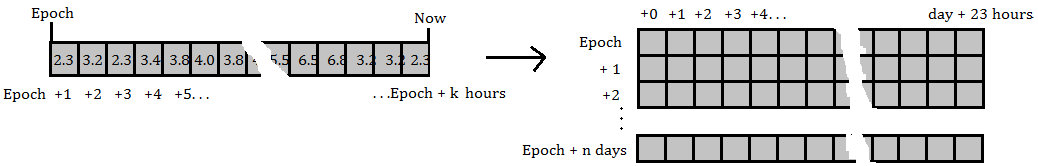
\includegraphics[scale=0.5]{illustrationofvector.png}
\caption{Illustration of feature extraction}
\end{figure}

Each row will thus correspond to a feature vector for a given day, where the 24 features are the hourly measured consumption during that day. Now for each day extra features are extracted and appended as extra columns to the original matrix. Table 5.7 shows a full list of the features that are extracted from the raw consumption figures of each day. 
\begin{figure}
\begin{center}
\begin{tabular}{|l | l | r |}
\hline
Feature & Description & Feature number \\ \hline
raw\_consumption & The raw hourly consumption figures during the day & 1-24 \\ \hline
mean & Average hourly consumption across entire day & 25 \\ \hline
peak & Maximum consumption observed for one hour&  26\\ \hline
min & Minimum consumption observed for one hour &  27\\ \hline
night & Average hourly consumption between 00:00 and 03:00 & 28 \\ \hline
morning & Average hourly consumption between 06:00 and 12:00 & 29 \\ \hline
afternoon & Average hourly consumption between 12:00 and 18:00 & 30 \\ \hline
evening & Average hourly consumption between 18:00 and 00:00 & 31 \\ \hline
mean/peak & The ratio between features mean and peak & 32\\ \hline
min/mean & The ratio between features min and mean&  33\\ \hline
night/day & The ratio between features night and day&  34\\ \hline
time\_of\_peak & At which hour does the daily peak occur& 35 \\ \hline
hours\_above\_mean & For how many hours is the consumption above the daily mean &  36\\ \hline
no\_of\_peaks & How many peaks occur during the day &  37\\ \hline
day\_of\_week & Categorical features indicating day of week& 38 \\ \hline
date & The date for when these measurements were observed &  39\\
\hline
\end{tabular}
\end{center}
\caption{Table of different features index}
\end{figure}
Each feature is easily calculated in R by applying various arithmetic functions to each row of the matrix. Each feature is then appended as an extra column to that matrix, resulting in a final matrix with 39 columns. Columns 1 to 24 contain the raw consumption measures, while the extracted features occupy the other columns.
Now when looking at an entire column alone, it can be considered a time serie itself with daily resolution. For instance column 25 will be a time serie of the average hourly consumption for each day since the \emph{epoch} setting. Column 26 will be the peak consumption recorded for each day, and column 28 the average hourly consumption at night. Thus each column is considered a time serie in itself and is stored as an array in the \emph{W\_Feature} table along with ids for the building and consumption type (\emph{water, electricity or heat}) that it describes. Thus the website can access this table to fetch time series showing the progression of various features for the buildings.
\section{Creating consumption profiles}
To extract further information from the data a number of consumption profiles are calculated. The consumption profiles can be viewed mainly as two parallel vectors where one is the mean values of certain features, while the other contains the standard deviations for these means. Consumption profiles are generated on 3 different levels, and the procedures to generate them are only run once a week rather than daily. 
\section*{Building profiles}
A building profile is generated for each building and consumption type if there is enough data to do so. These profiles will contain the means and standard deviations of features 25 to 37. Thus a building profile summarizes data about a building's consumption patterns by calculating means and standard deviations for the various feature time series described in previous section. Thus a building profile would for instance contain data about the overall averages and standard deviations for a buildings hourly consumption, night consumption, day vs. night consumption ratio etc. The building profiles are then stored in the \emph{W\_Building\_Profiles} table, ready for the website to access.
\section*{Subtype profiles}
The subtype profiles are created by grouping building profiles which belong to buildings of the same subtype (eg. schools, offices, nursing homes etc). Combining the means (my) and standard deviations $s$ would normally be done with the formulas in figure 5.8, where $n$ is the number of observations in each sample, which would be the number of days.
\begin{figure}
\begin{center}
$\mu = \frac{\mu_1\cdot n_1+\mu_2\cdot n_2+ \cdots +\mu_k\cdot n_k}{n_1+n_2+ \cdots +n_k}$
\newline
\newline
$S_w^2 = \frac{(n_1-1)s_1^2+(n_2-1)s_2^2+\cdots +(n_k - 1)s_k^2}{n_1 + n_2+\cdots +n_k -k}$
\end{center}
\caption{Subtype Profiles equation}
\end{figure}

However, this approach is not used since we are not interested in the combined mean and standard deviation for each day across different buildings, but rather we will calculate new means and standard deviations using the means found in the building profiles as input. The subtype profiles are then saved in table \emph{W\_Subtype\_Profiles}.
\section*{Daytype profiles}
When it comes to energy and water consumption most buildings will have at least two different day types; workdays and weekends. On each type of day the consumption will follow a distinct pattern. For each building the distinct day types are identified, and a daytype profile modelling the consumption pattern is created. The day type profiles are created in four steps which include preprocessing, LDA, clustering and outlier detection. The matrix containing features for each day since epoch as explained in section \emph{Extracting features}, is the input for these processing steps.
\subparagraph{Preprocessing:}Two adjustments are done in order to make similar days easier to detect. First the seasonality is removed by subtracting the minimum consumption for each day. Second, because all observation times are measured in GMT time, observation values measured during winter time are shifted one hour later. Otherwise the feature vectors of winter time days and summer time days would become out of sync, as people's routines would be one hour earlier during winter time. 
\subparagraph{Outlier detection:}Using the PCout multivariate outlier detection algorithm\footnote{See Related work and Outliers}  extreme outliers are removed from the dataset. The algorithm is applied to features 25, 26 and 27 (mean, peak and min), as at least one of them will be affected directly by an extremely high or low observed value at any given time during the day. It is important to remove outliers before performing LDA, because it is not a robust statistical method, and can potentially be highly affected by outliers.
\subparagraph{LDA:}Because the dataset is large, it is important that the optimal number of day types to use for each building, and the best features to use for the grouping are selected automatically. Based on the knowledge that similar consumption patterns mostly occur on the same day of the week, a linear discriminant analysis (LDA) was performed to find the linear combinations of features 25 to 37 that give the best separation between the classes. The maximum number of useful discriminant functions is the minimum of G-1 and p where G is the number of groups and p the number of features. Thus the LDA resulted in 6 different linear combinations of the features that could best separate the days of the week, and thus also different types of days as those will most often be on the same day of the week. Using the linear discriminant functions from the LDA, each day’s features 25 to 37 were reduced into 6 features called canonical variates (CV’s).
\subparagraph{Clustering}Based on the CVs of each day a k-medoids clustering was performed. K-medoids was chosen over k-means because it performed well, and the implementation pamk in the R package fpc automatically detects the optimal number of clusters using the optimum average silhouette width which is a measure of how well the data is clustered \cite{PeterJRousseeuw}. 

Once similar days have been clustered, a day type profile is created for each cluster. This is done by finding means and standard deviations for features 1 to 37 and putting them in two parallel arrays. These arrays along with the building id and consumption type would be stored in the W\_Consumption\_Profiles table. An array of length 7 is also stored, which indicates the occurrences of each weekday in this pattern. Additionally a weight for each profile is computed as ($\frac{total\_days}{days\_in\_cluster_n}$)	. For instance if 200 days were initially used for the clustering and clusters A and B were created with 50 and 150 days respectively, then two day type profiles would be created with weights 0.25 and 0.75.
\section{Comparing buildings}
To identify buildings with similar consumption patterns the daytype profiles are used rather than the building profiles. The system uses an approach similar to the K Nearest Neighbor method to find similar daytype profiles. Figure 5.9 illustrates with a fictitious example how using the daytype profiles is different from using the building profiles to compare buildings. In figure 5.9 a) 5 daytype profiles belonging to 3 buildings are shown in a two dimensional space (each profile is assumed to be of equal weight here). Building 1 and 3 have two day type profiles each which are located pairwise near each other, while Building 2 only has 1 day type profile. Now using proximity as a measure of similarity we can see in b) that if we compare based on the daytype profiles Building 1 and 3 would be similar to each other. If we average the day type profiles belonging to the same building we would have essentially the building profiles. Figure 5.9 c) shows that if those were used for comparing that now Building 1 and 2 would appear similar. 
\begin{figure}
\begin{center}
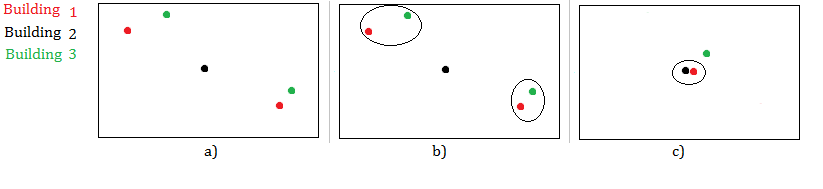
\includegraphics[scale=0.5]{buildingsimmilarity.png}
\end{center}
\caption{Building similarity}
\end{figure}
This demonstrates that the two approaches render different results, and that by using the building profiles two buildings with very different consumption patterns can appear to be similar because of the averaging of features. Thus the comparison is done based on all the daytype profiles for each building.

First a distance matrix between all day type profiles is computed using euclidean distances. The same canonical variates used for clustering are used to compute the distances. The smaller the distance the more similar the profiles will be. However as day type profiles only partly represent the full consumption pattern of their buildings, both each row and each column is divided by the weight of the profile at that row or column. This means that each measure of distance in the matrix is adjusted by the weights of both the two profiles being compared. For each building the distances across all its profiles to other profiles are summed. Then picking the profiles with lowest distance measure will be for the buildings that are most similar. The 30 profiles with lowest distance are picked out and the ids of the buildings behind those profiles are stored in an array which is saved to the \emph{W\_Similar} table from where the website can access the results.
\section{Detecting faults}
The detection of faults is based on the assumption that day days of similar types have variables that are each normally distributed. This assumption has been verified using a QQ-plot. The daytype profiles contain means and standard deviations of all variables for each type of day. With this information the following hypothesis test can be constructed for any daytype profile type and a given day
\begin{itemize}
\item $H_0$:\emph{day} is of \emph{type}
\item $H_A$:\emph{day} is not of this \emph{type}
\end{itemize}
A two tailed hypothesis test is then performed using Z-scores to get the p value of this hypothesis test. First the Z score of each variable i is computed with:
\begin{center}
$Z_i=\frac{x_i-\mu_i}{\sigma_i}$
\end{center}
where $x_i$ is the value of variable i for day, $\mu_i$ and $\sigma_i$ is the mean and standard deviation of variable i from the daytype profile. With the Z score the p value $\pi$ for variable $i$ can be calculated for the two tails as illustrated in figure 5.10:
\begin{figure}
\begin{center}
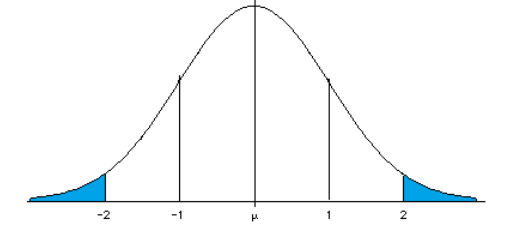
\includegraphics[scale=0.5]{normalDist.PNG}
\end{center}
\caption{Two tailed cutoff on normal distribution}
\end{figure}
To get the total p value $p_{total}$ across all variables the following equation is used:
\begin{center}
$p_{total}=\displaystyle\prod_{i=1}^N p_i$
\end{center}
where $N$ is the total number of variables.

The significance level $\alpha$ indicates when to reject $H_0$ and say that a given day does not conform to a certain day type profile. A low $\alpha$ would decrease the chance of false alarms but decrease the chance that true anomalies are detected (ie. the chance of making type 2 errors increase). On the other hand a high $\alpha$ value increases the chance of detecting anomalies, but potentially increases the number of false alarms (ie. type 1 errors). $H_0$ is rejected when following equation evaluates to true:
\begin{center}
$p_{total} <\alpha^N$
\end{center}
where $N$ is the total number of features.

If all $H_0$ is rejected for all day type profiles the tested day is considered an anomaly, and the variable with lowest p value is flagged as a probable cause. The reason why a day is checked against every daytype profile individually rather than against a single building profile, is because the hypothesis test assumes that the means and standard deviations of variables come from a normal distribution. This would not be the case if a building's consumption comes from two or more distinct day types that each have normally distributed variables with different means and standard deviations. This is illustrated in figure 5.11, where two different normal distributions are plotted together, showing that the result is not normally distributed.
\begin{figure}
\begin{center}
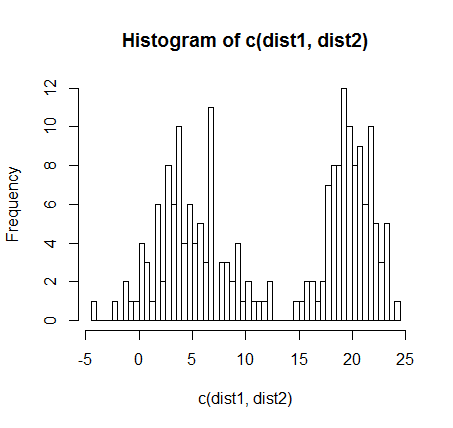
\includegraphics[scale=0.4]{histogramnormaldists.png}
\end{center}
\caption{Two different normal distributions}
\end{figure}

The features to use to detect anomalies and the $\alpha$ value can easily be configured by users through the website as the settings are stored in the \emph{W\_Settings} table. This will allow users to tweak the power of the test. The standard configuration is to use $\alpha$ 0.5 and two features, the average consumption across the entire day and the consumption at night. The first feature will detect an anomaly if the total consumption goes up or down for any reason, while the night consumption feature would be particularly sensitive if standby consumption of a building changes. When an anomaly is detected an alarm is created and stored in the \emph{W\_Alarm\_Odd\_Consumption} table, where it can be accessed by the website.
\newline
\section{Design of the website}
This section will describe the design of the website. It will clarify which perspectives have been in focus, what technologies have been used. Lastly will it describe the different elements of the website.

The use case diagram from the Requirements section gives an overview of the requirements. Further does it show a grouping of the requirement into two main concepts: \emph{Viewing a building} and \emph{Comparing}. In relation to user interface design Steve Krug, argues that clearly defined areas and hierarchies aids the users learnability of a system and supports from getting lost \cite{interaction}. Based on this, these identified concepts become important for the organization user interface, as these concepts can serve as groupings. Since the website should provide the user with a considerable amount of information, ordering and displaying it in a simple way becomes important.

In addition, each of the use cases relates to different purposes when using the system. In order to keep it simple and support the user in quickly gaining access to the information needed to perform a certain task, keeping each sub use case visually apart from each other may ease the navigation. Furthermore, by keeping them apart is it possible differ their appearance and thereby making them more memorable for the user and minimizing the risk of a user confusing/mixing up information presented.
\section*{Viewing a building}
The one thing all use cases of viewing a building have in common is that they, to a certain extend only display information, and require little or no interaction from the user. Based on the findings from the previous section and with this in mind, it has been decided create and display each use case in separated bordered panels that clearly encapsulate and separates them.
\section*{Comparing buildings}
Comparing buildings, in contrast to viewing a single building, requires a higher level of interaction from the user. Further, the first four use cases can be generalized into a concept of \emph{what to compare}, and the last can be viewed as \emph{how to compare}. This generalization, enhance the flexibility of the system, since it allows buildings, types and categories to be treated as one. Doing this, will allow comparison between buildings and types, categories and types or categories and buildings with a uniform GUI. With a uniformed GUI for the four types of content to compare, the number of steps the user have to learn is minimized, making it easier to learn, but also easier to remember. Based on this it is now possible to define three areas of the page:
\begin{itemize}
\item The content to compare.
\item The features on which the user compare content.
\item The visualization of the comparison.
\end{itemize}
In order to clarify the placement of these areas Jeffrey Venn extension to Keith Instone theory of the fundamental visibility of a system have been used \cite{interaction}. Jeffrey Venn extension associates Keith Instones three question (\emph{Where am i?, What is here? and Where can i go?}) with three areas on a page. In relation to this the content to compare have been associated with \emph{Where can i go?}, to encourage the user to explore the data. Since the \emph{Where am i?}, continuously throughout the website is have been allocated for navigation and information about where on the website the user is, the features to compare have been chosen to be put into main content area along with the visualization of the comparison. These two sub areas of the main content area, have been clearly divided, but still placed close together to insure the user catches the relation between them.
\section*{Flow of website}
Based on the concepts and their hierarchy, discovered in previous section, the flow of the website was developed see figure 5.12. The page Building and Compare are directly causes of the groupings into hierarchies discovered, whereas the alarm pages originates from requirement \emph{F3-02}\footnote{See requirement specification.}. The homepage have been created as an control and navigation page. In addition, the requirement specification expresses a need for user policies and restricted access to some features, like validation of data and handling of alarms. In order to accommodate these requirements the login and signup page have also been added.
\begin{figure}
\begin{center}
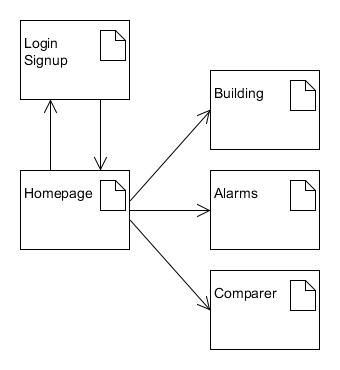
\includegraphics[scale=0.3]{FlowDiabramWebSite.jpg}
\end{center}
\caption{Flowchart of the website}
\end{figure}
\section{Implementation of website}
\section*{Template panels and visual components}
As mentioned previously, as a design choice, it have been chosen to visibly keep different functionality clearly apart. From a system design perspective, standardizing these functionalities into components gives the software system have many advantages. Firstly, the system becomes more flexible and enhance the possibilities for code reuse. Further, by standardizing how components are created lowers complexity and easen development at a later state in the software life cycle. In addition, by standardizing reusable components the system becomes more easily changeable. Lastly by creating a “toolbox” with standard components, the view and display of information is more easy to customize to the user, if for example different users should have different views of the information. Further does it allow for generalizing functionality for collapsing, closing and reorganizing different elements on a given page.  

For these reasons it have been chosen to design and implement a simple template framework (working as a factory pattern), where a controlling module contains a list of templates and how to instantiate them. Furthermore does the template framework contain a class which all templates extends. As seen in figure 5.13, an instance of the Template object contains a link or references to a HTML part. When an instance is created this HTML part is firstly cloned, and then filled out by the instance object with the provided data. The instance object, besides how to fill out the HTML, also contains all functionality regarding behavior and events. Lastly, to reduce coupling and make each component independent of other components all intercommunication between components is intended to work through events.

Besides this template framework, to ensure a rapid development of the prototype a number of libraries and technologies have been used.
\begin{figure}
\begin{center}
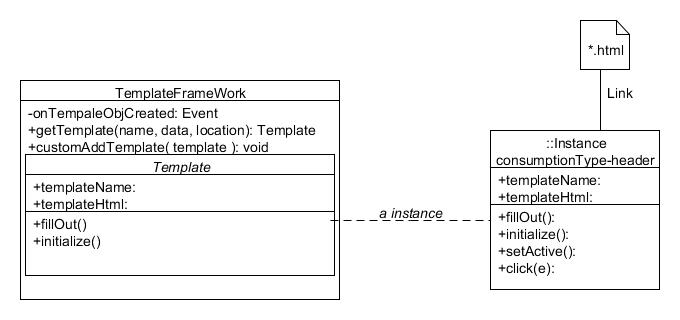
\includegraphics[scale=0.3]{W_template_eksample.jpg}
\end{center}
\caption{Template framework}
\end{figure}
\section*{Technologies}
Firstly, as some of the most commonly used, JQuery\footnote{https://jquery.com} and Bootstrap\footnote{http://getbootstrap.com} have been integrated. JQuery have been used to lessen the code needed to be written and to more easily handle events and animations. Further the Bootstrap framework for styling and in order to make the application more responsive and lean towards a mobile first development to ensure portability.  
In order to create visualizations of the data the D3\footnote{http://d3js.org/} (Data Driven Documents) library have been used. Lastly for backend and client communication Dream Factory\footnote{https://www.dreamfactory.com/} have been used. This open source platform, does with little configuration, create a RESTful service and API to database. Thereby enabling the front end application to get and set data from the database through the API. 
After a session have been established, through a login (either by an anonymous or by a registered user profile) data can be retrieved the client SDK. 

The code snippet in figure 5.14 shows how the Comparing buildings page gets data for the charts.
\begin{figure}
\begin{center}
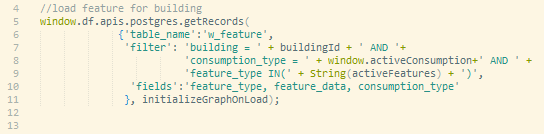
\includegraphics[scale=0.85]{codesnippet.png}
\end{center}
\caption{Code snippet of how to retrieve data}
\end{figure}
The \emph{getRecords} method takes two parameters: an object containing information of what to retrieve and where to retrieve it, and a callback-function.
The object-parameter has numerous configuration parameters. Mainly, in the implementation of the web-site, only three is used (\emph{table\_name, fields and filter}), which specifies the content of a basic SQL select-statement.
\newline
\newline
For further description of the implementation of the website see Appendix 06 -Implementation of the Website. This appendix discuss the implementation of the requirements on the website, the structure of the HTML and the relation between the different  HTML files and JavaScripts files.


